\section{Conclusion}
\label{Chap:Al/Vac:section:Conc}


In this chapter, Ag-Mg-Zn ternary alloy is used as a model system to simulate the solute clustering kinetics in Al 7000 series alloys. We first demonstrate that the \acf{BEP} relationship, which suggests a simple linear relation between the activation barrier and the reaction energy of one elementary reaction step, fails to provide quantitatively accurate migration barriers of vacancies in these multi-component Al alloys. Then we develop a \ac{NN} model to predict vacancy migration barriers using the training data set of thousands of \ac{DFT} calculated barriers for different alloy configurations. A \ac{kMC} method based on this \ac{NN} model is used to study the early transition behavior from a supersaturated solid solution to solute clusters and \acf{GP} zones in Al-Mg-Zn alloys. A local super-basin method  \ref{Chap:Al/Vac:sec:LSKMC}, together with \ac{LRU} cache \ref{Chap:Al/Vac:sec:LRU}, is also implemented to accelerate \ac{kMC} simulations. We also propose a pseudo-atoms approach to efficiently search the alloying strategy to slow down the solute clustering and the corresponding natural aging effects in Al 7000 series alloys. In this approach, a small number of pseudo-atoms with artificially designed ability to change vacancy migration barriers are added into the Al matrix, and the \ac{kMC} simulations are performed to check their effects to clustering kinetics (so-called "sensitivity test"). We also develop the quantitative analysis methods to describe the chemical and structural properties of clusters. At last, we propose a machine learning strategy based on the structural and chemical information of clusters and precipitates from \ac{kMC} simulations to predict the cluster strengthening and natural aging effects in future studies.


\newpage
\begingroup
\begin{figure}[!ht]
  \centering
  \subfigure[$\varepsilon_{Mg-X} = 0.05$, cluster]{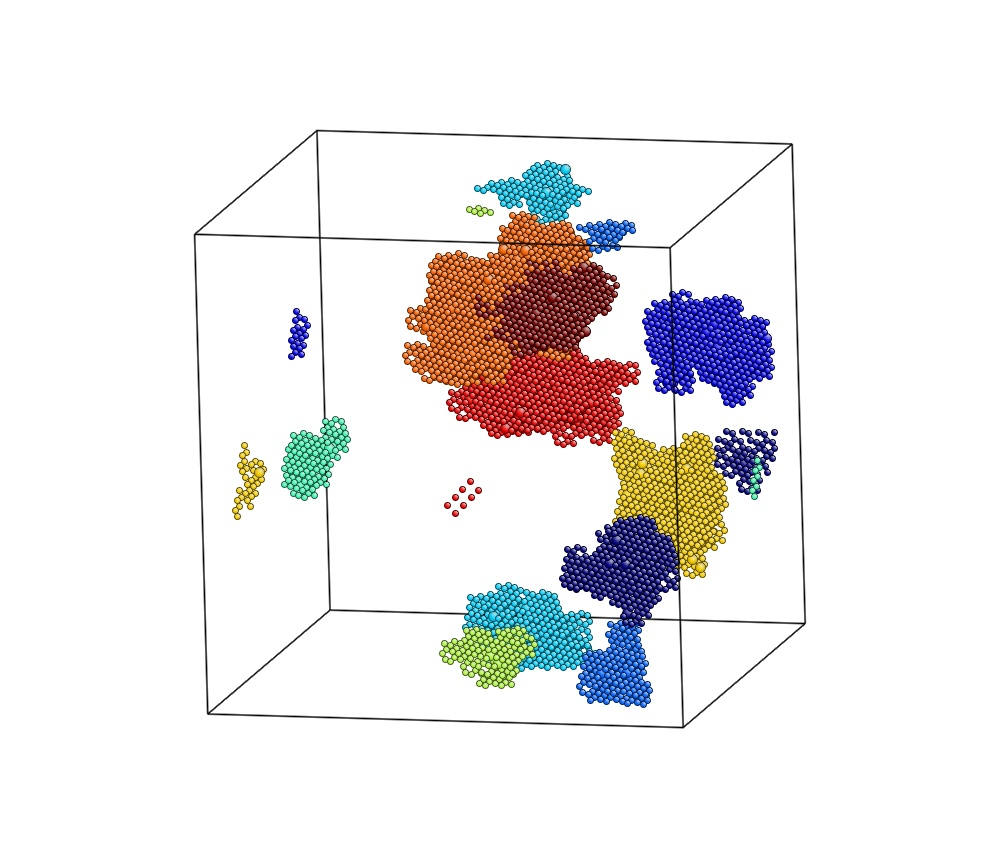
\includegraphics[width=0.49\linewidth]{Chap5/plots/cluster_id_jpg/00003.jpg}}
%   \subfigure[control]{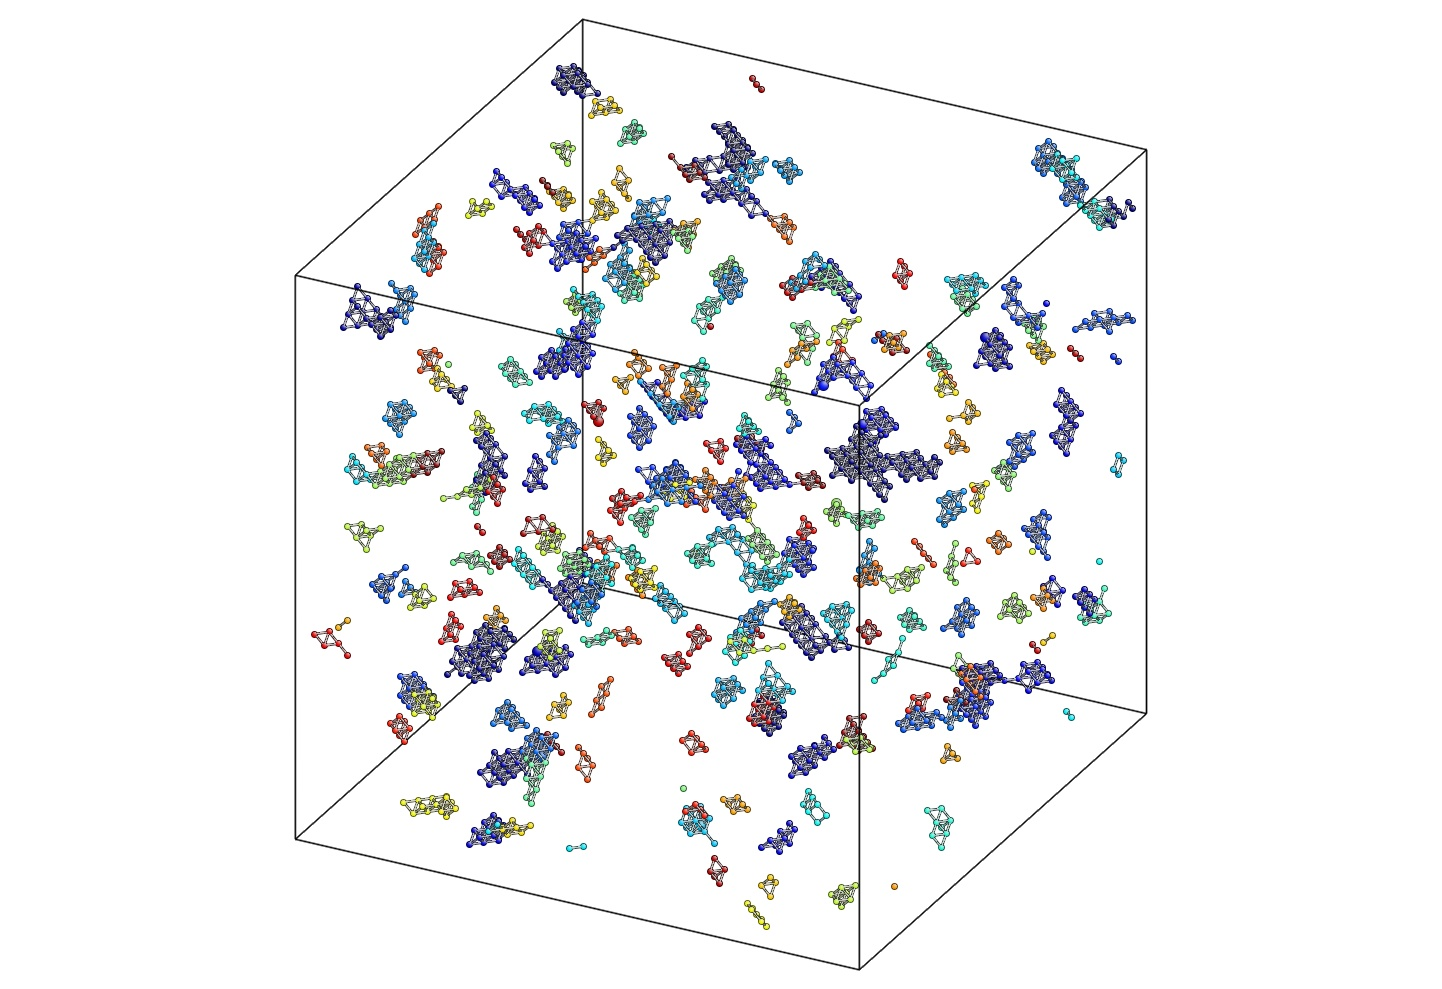
\includegraphics[width=0.32\linewidth]{Chap5/plots/cluster_id_jpg/00000.jpg}}
  \subfigure[$\varepsilon_{Mg-X} = -0.05$, cluster]{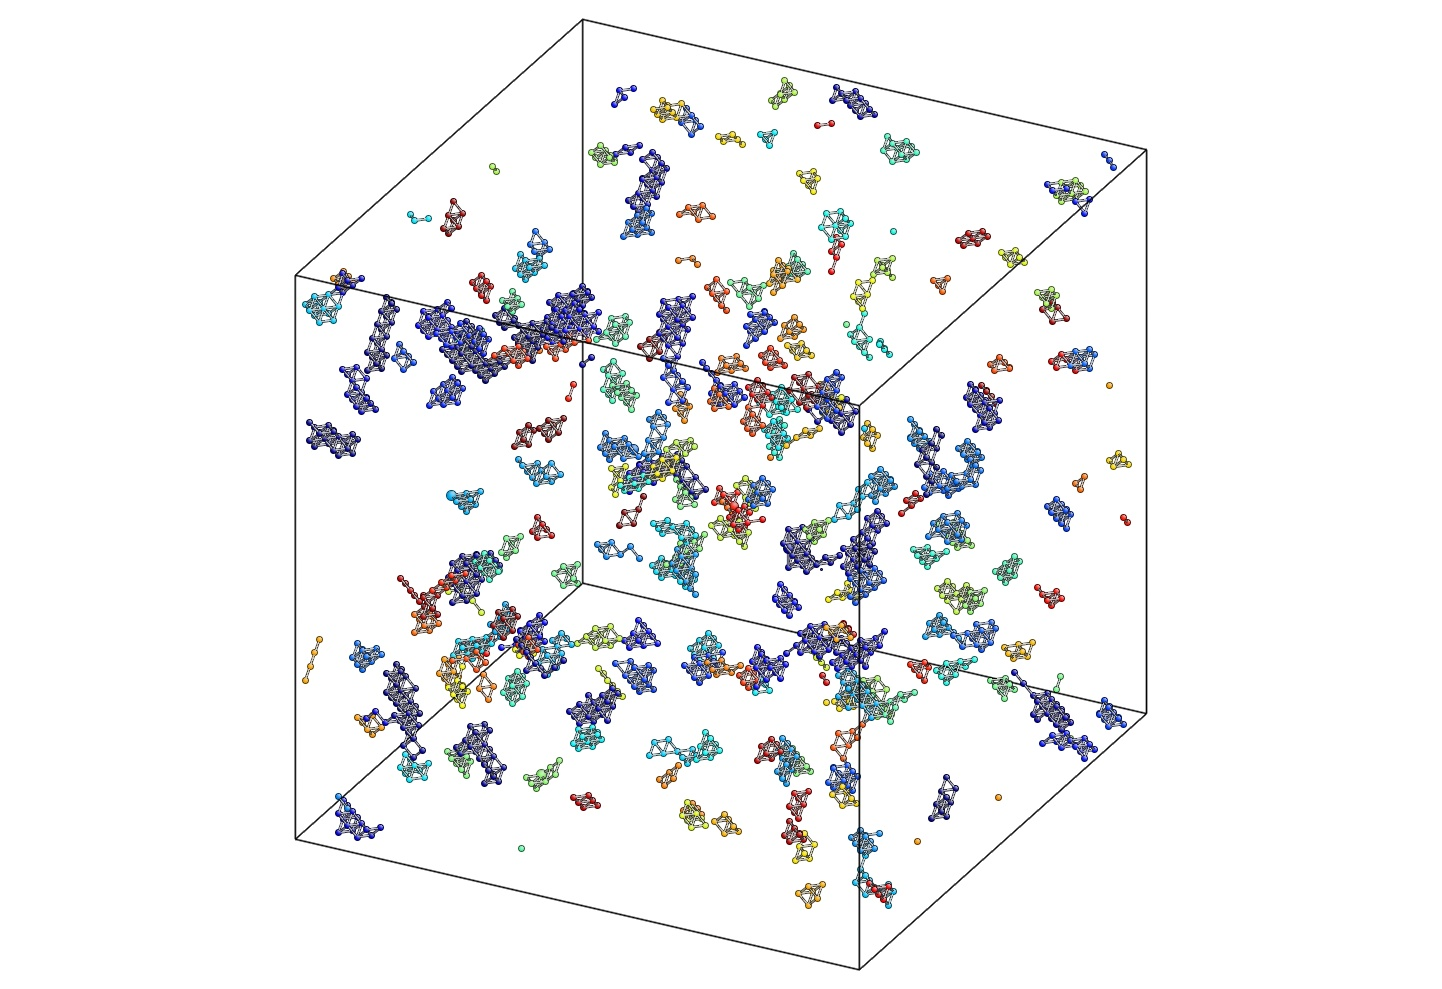
\includegraphics[width=0.49\linewidth]{Chap5/plots/cluster_id_jpg/00004.jpg}} \\
  \subfigure[$\varepsilon_{Mg-X} = 0.05$, species]{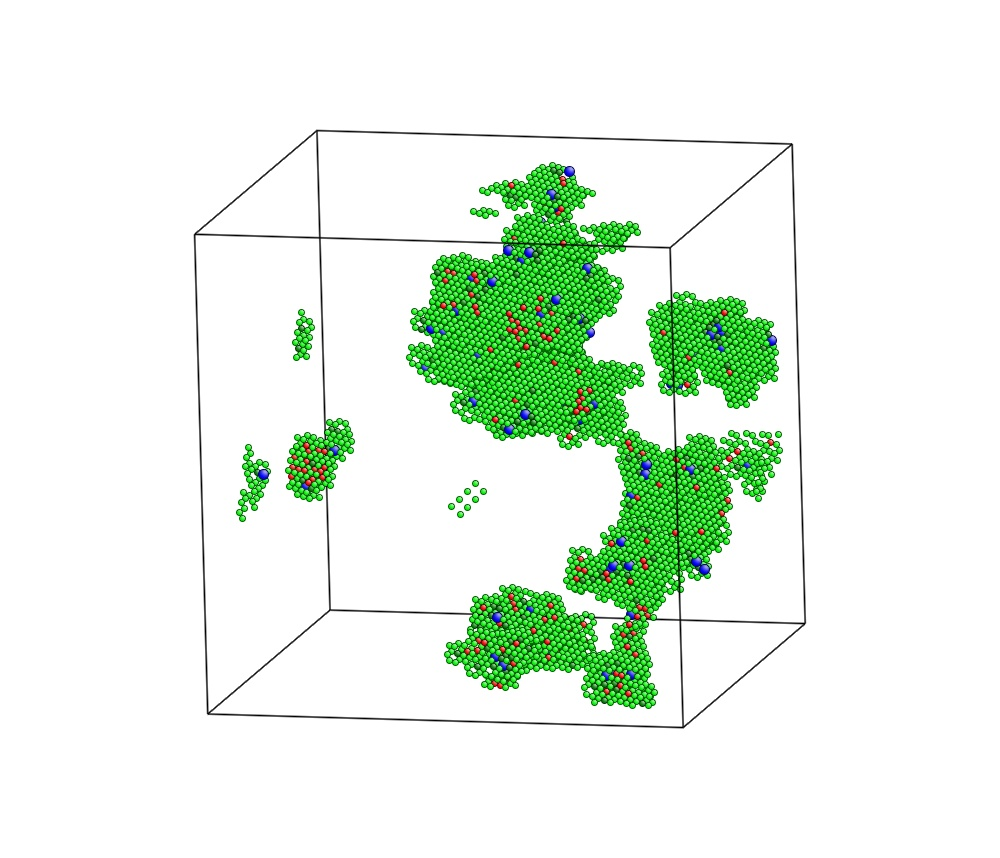
\includegraphics[width=0.49\linewidth]{Chap5/plots/element_jpg/00003.jpg}}
%   \subfigure[control]{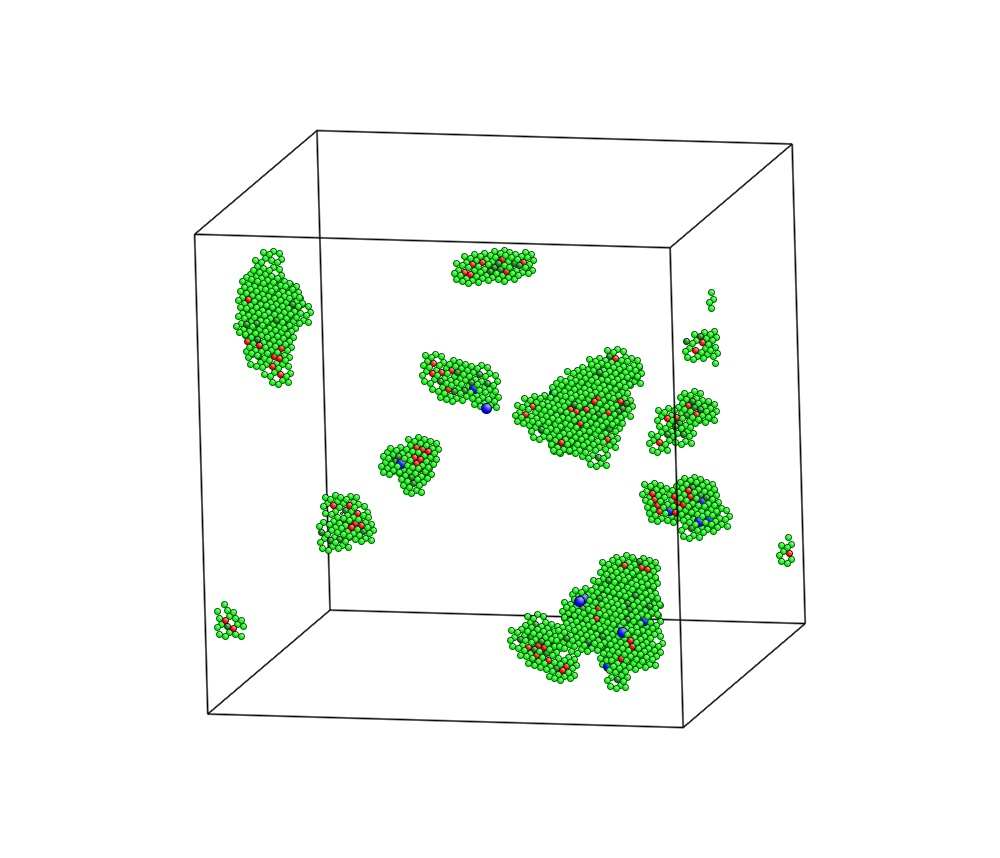
\includegraphics[width=0.32\linewidth]{Chap5/plots/element_jpg/00000.jpg}}
  \subfigure[$\varepsilon_{Mg-X} = -0.05$, species]{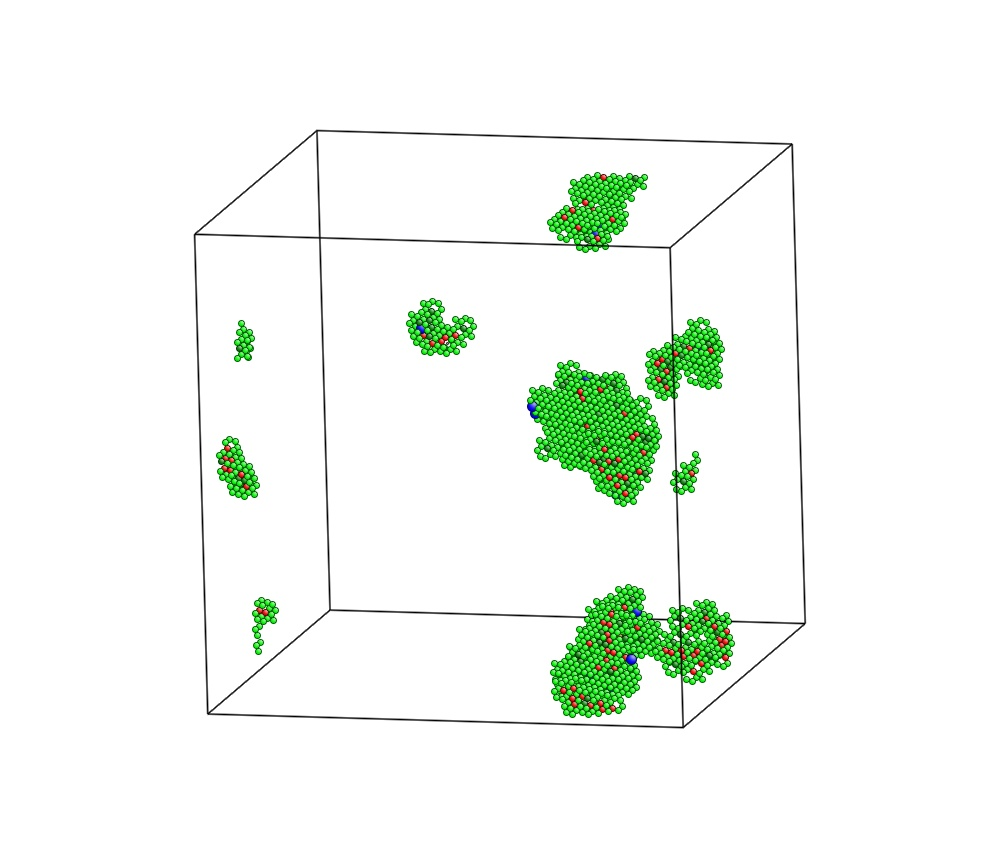
\includegraphics[width=0.49\linewidth]{Chap5/plots/element_jpg/00004.jpg}}
% \caption[Atomistic pictures of 108,000 atoms for $\varepsilon_{Mg-X}$ sensitivity test.]{Atomistic pictures of 108,000 atoms for $\varepsilon_{Mg-X}$ sensitivity test. (a), (d) : $\varepsilon_{Mg-X} = 0.05$, which is setup \#3 in Table \ref{Chap:Al/Vac:tab:pseudo1}. (b), (e) : setup \#0 in Table \ref{Chap:Al/Vac:tab:pseudo1}. (c), (f) : $\varepsilon_{Mg-X} = -0.05$, which is setup \#4 in Table \ref{Chap:Al/Vac:tab:pseudo1}. (a), (b), and (c) are colored by cluster size. The color mapping from dark blue to red is ranked by the cluster size in descending order. (d), (e), and (f) are colored by atom species.  Light green, dark green, red, and blue atoms are Al, Mg, Zn, and pseudo atoms respectively.}
\caption[Atomistic pictures of 108,000 atoms for $\varepsilon_{Mg-X}$ sensitivity test.]{Atomistic pictures of 108,000 atoms for $\varepsilon_{Mg-X}$ sensitivity test. (a), (c) : $\varepsilon_{Mg-X} = 0.05$, which is setup \#3 in Table \ref{Chap:Al/Vac:tab:pseudo1}. (b), (d) : $\varepsilon_{Mg-X} = -0.05$, which is setup \#4 in Table \ref{Chap:Al/Vac:tab:pseudo1}. (a) and (c) are colored by cluster size. The color mapping from dark blue to red is ranked by the cluster size in descending order. (b) and (d) are colored by atom species. Light green, dark green, red, and blue atoms are Al, Mg, Zn, and pseudo atoms respectively. And small gray sticks are bonds between atoms.}
\label{Chap:Al/Vac:fig:sens_Mg}
\end{figure}
\endgroup

\newpage
\begingroup
\begin{figure}[!ht]
  \centering
  \subfigure[$\varepsilon_{Zn-X} = 0.05$, cluster]{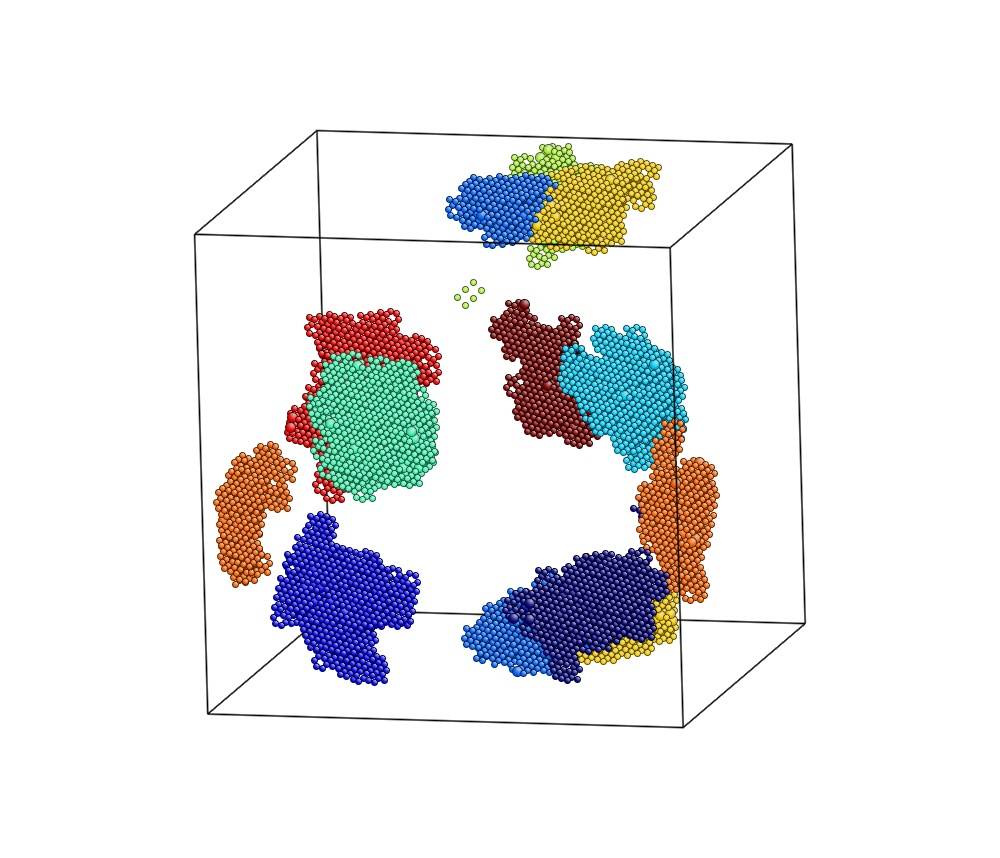
\includegraphics[width=0.49\linewidth]{Chap5/plots/cluster_id_jpg/00005.jpg}}
%   \subfigure[control]{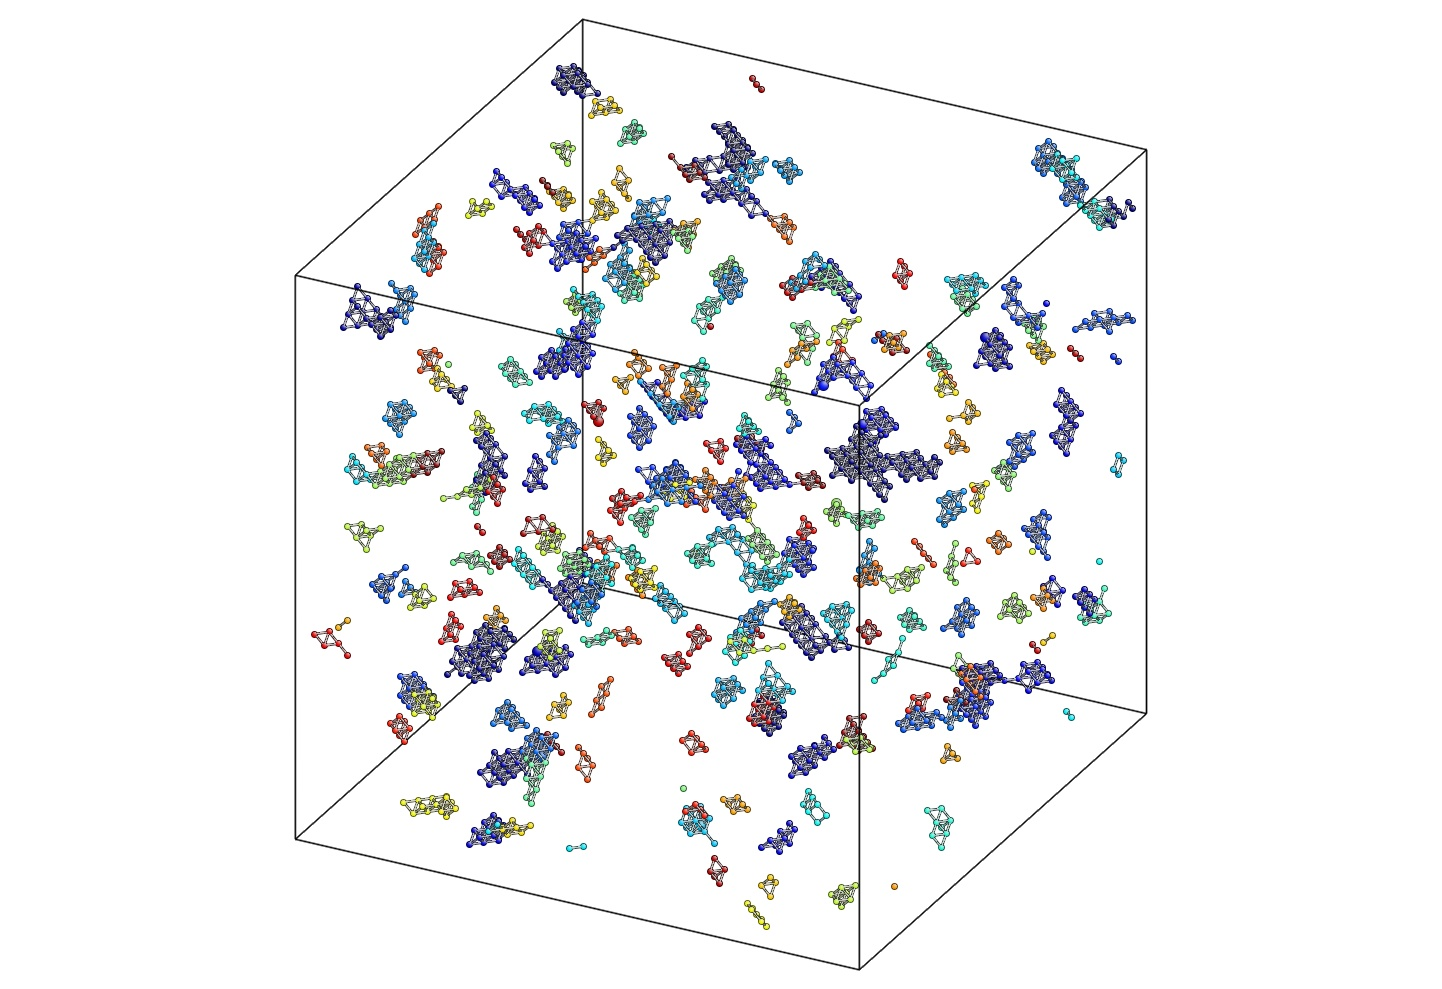
\includegraphics[width=0.32\linewidth]{Chap5/plots/cluster_id_jpg/00000.jpg}}
  \subfigure[$\varepsilon_{Zn-X} = -0.05$, cluster]{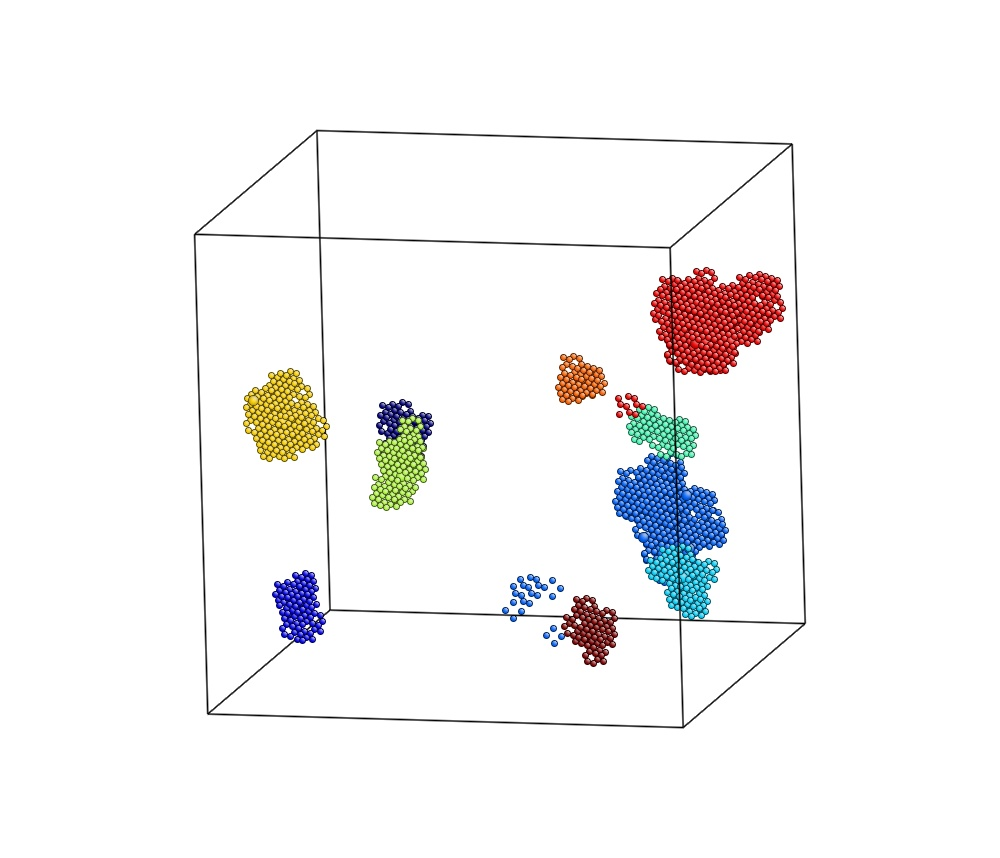
\includegraphics[width=0.49\linewidth]{Chap5/plots/cluster_id_jpg/00006.jpg}} \\
  \subfigure[$\varepsilon_{Zn-X} = 0.05$, species]{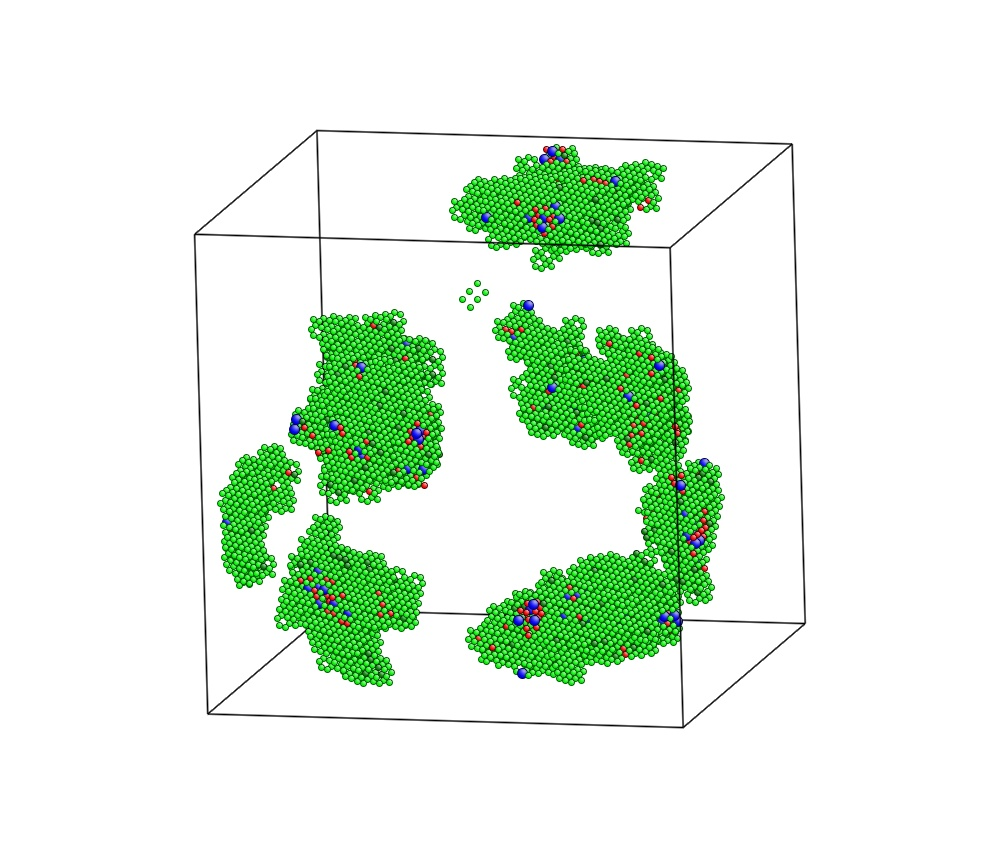
\includegraphics[width=0.49\linewidth]{Chap5/plots/element_jpg/00005.jpg}}
%   \subfigure[control]{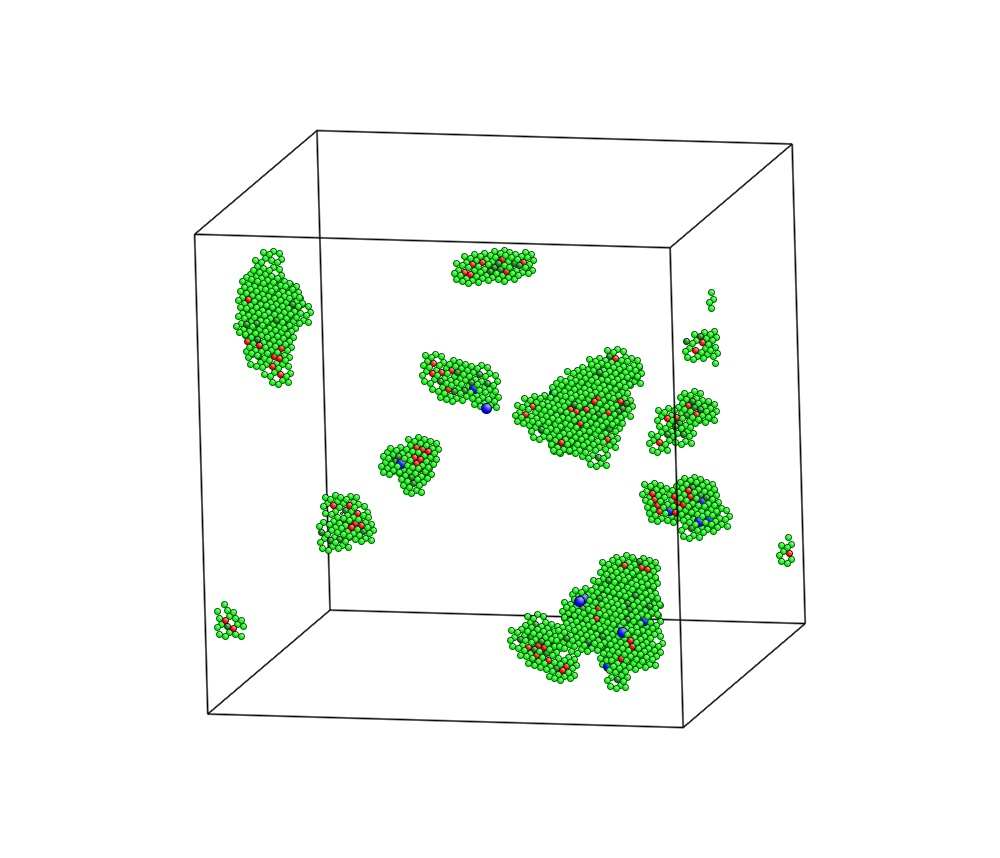
\includegraphics[width=0.32\linewidth]{Chap5/plots/element_jpg/00000.jpg}}
  \subfigure[$\varepsilon_{Zn-X} = -0.05$, species]{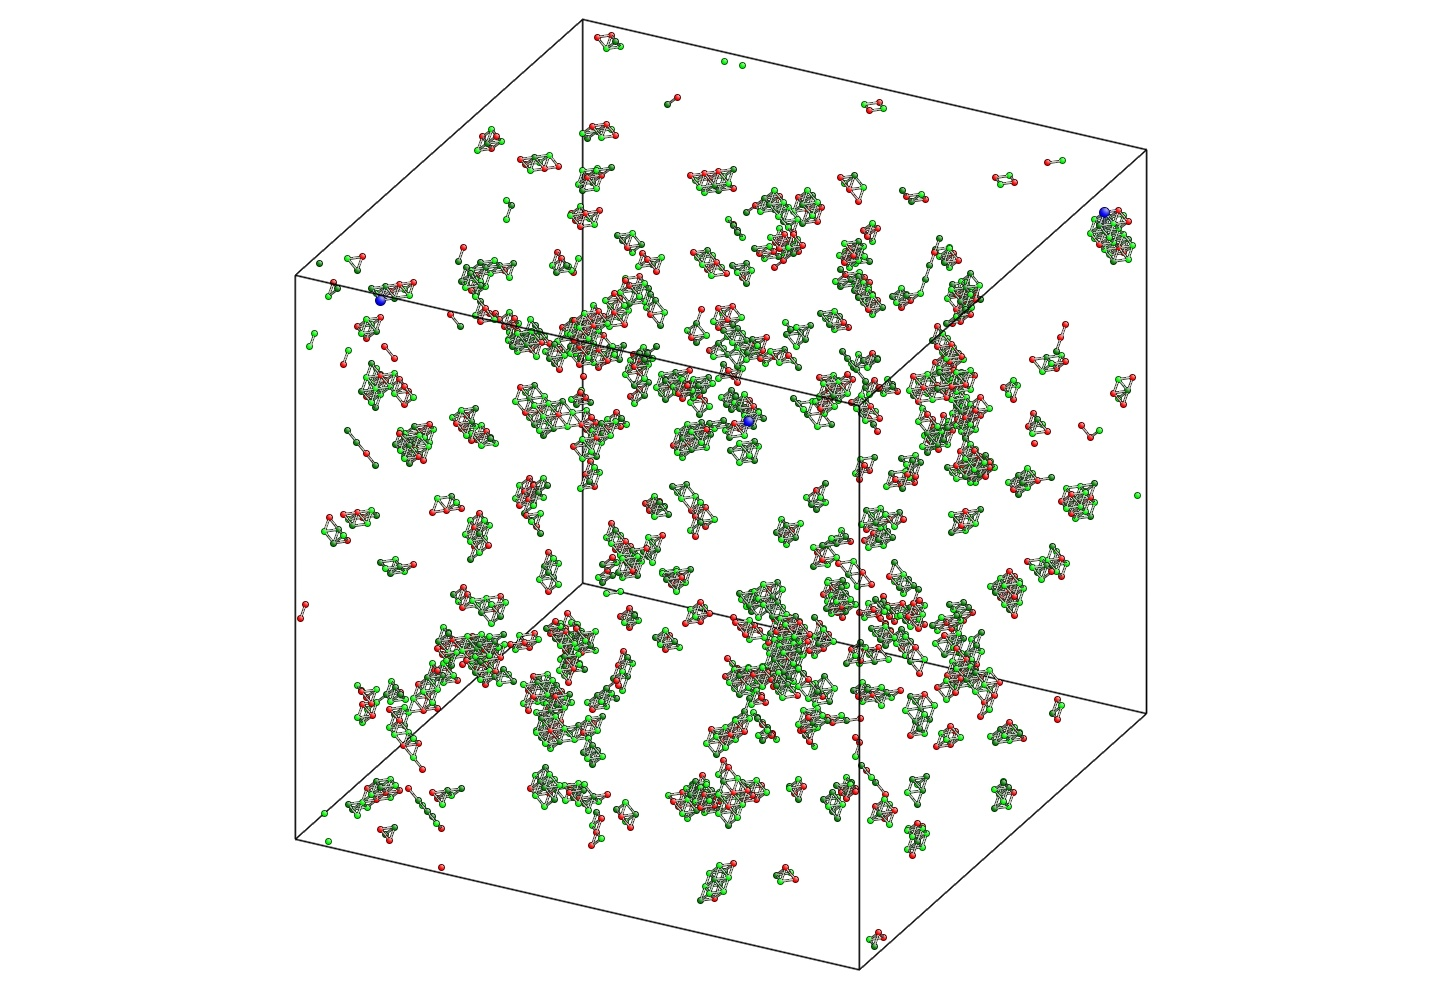
\includegraphics[width=0.49\linewidth]{Chap5/plots/element_jpg/00006.jpg}}
% \caption[Atomistic pictures of 108,000 atoms for $\varepsilon_{Zn-X}$ sensitivity test.]{Atomistic pictures of 108,000 atoms for $\varepsilon_{Zn-X}$ sensitivity test. (a), (d) : $\varepsilon_{Zn-X} = 0.05$, which is setup \#5 in Table \ref{Chap:Al/Vac:tab:pseudo1}. (b), (e) : setup \#0 in Table \ref{Chap:Al/Vac:tab:pseudo1}. (c), (f) : $\varepsilon_{Zn-X} = -0.05$, which is setup \#6 in Table \ref{Chap:Al/Vac:tab:pseudo1}. (a), (b), and (c) are colored by cluster size. The color mapping from dark blue to red is ranked by the cluster size in descending order. (d), (e), and (f) are colored by atom species.  Light green, dark green, red, and blue atoms are Al, Mg, Zn, and pseudo atoms respectively.}
\caption[Atomistic pictures of 108,000 atoms for $\varepsilon_{Zn-X}$ sensitivity test.]{Atomistic pictures of 108,000 atoms for $\varepsilon_{Zn-X}$ sensitivity test. (a), (c) : $\varepsilon_{Zn-X} = 0.05$, which is setup \#5 in Table \ref{Chap:Al/Vac:tab:pseudo1}. (b), (d) : $\varepsilon_{Zn-X} = -0.05$, which is setup \#6 in Table \ref{Chap:Al/Vac:tab:pseudo1}. (a) and (c) are colored by cluster size. The color mapping from dark blue to red is ranked by the cluster size in descending order. (b) and (d) are colored by atom species. Light green, dark green, red, and blue atoms are Al, Mg, Zn, and pseudo atoms respectively. And small gray sticks are bonds between atoms.}
\label{Chap:Al/Vac:fig:sens_Zn}
\end{figure}
\endgroup